\documentclass{standalone}
\usepackage{tikz}
\usetikzlibrary{calc,patterns,decorations.pathmorphing,decorations.markings}

\newcommand{\nvar}[2]{%
    \newlength{#1}
    \setlength{#1}{#2}
}

% Define a few constants for drawing
\nvar{\wheelh}{2cm}

\begin{document}

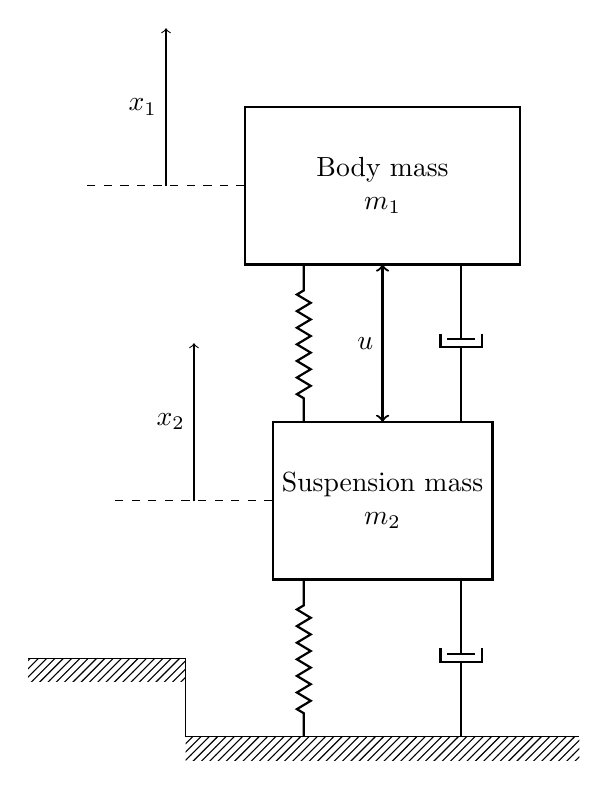
\begin{tikzpicture}[every node/.style={draw,outer sep=0pt,thick}]
\tikzstyle{spring}=[thick,decorate,decoration={zigzag,pre length=0.3cm,post length=0.3cm,segment length=6}]
\tikzstyle{damper}=[thick,decoration={markings,  
  mark connection node=dmp,
  mark=at position 0.5 with 
  {
    \node (dmp) [thick,inner sep=0pt,transform shape,rotate=-90,minimum width=15pt,minimum height=3pt,draw=none] {};
    \draw [thick] ($(dmp.north east)+(2pt,0)$) -- (dmp.south east) -- (dmp.south west) -- ($(dmp.north west)+(2pt,0)$);
    \draw [thick] ($(dmp.north)+(0,-5pt)$) -- ($(dmp.north)+(0,5pt)$);
  }
}, decorate]
\tikzstyle{ground}=[fill,pattern=north east lines,draw=none,minimum width=5cm,minimum height=0.3cm]


\node (M1) [align=center, minimum width=3.5cm,minimum height=2cm] {Body mass\\ $m_1$};
\node[align=center, below of=M1, node distance=4cm] (M2) [minimum width=2.5cm,minimum height=2cm] {Suspension mass\\ $m_2$};

\node[ground, below of=M2 ,anchor=north, node distance=3cm] (ground1) {};
\draw (ground1.north west) -- (ground1.north east);
\node[ground, left of=ground1, minimum width=2cm, yshift=1cm, xshift=-2.5cm] (ground2) {};
\draw (ground2.north west) -- (ground2.north east);
\draw (ground2.north east) -- (ground1.north west);

\draw [spring] (ground1.north) ++(-1cm, 0) -- ++ (0, 2cm);
\draw [damper] (ground1.north) ++(1cm, 0) -- ++(0, 2cm);

\draw [spring] (M2.north) ++(-1cm, 0) -- ++ (0, 2cm);
\draw [damper] (M2.north) ++(1cm, 0) -- ++(0, 2cm);

\draw[dashed, thin] (M2.west) -- ++(-2cm, 0) ++ (1cm, 0);
\draw[solid, , ->] (M2.west) ++(-1cm, 0) -- node[left, draw=none] {$x_2$} ++(0, 2cm);
\draw[dashed, thin] (M1.west) --  ++(-2cm, 0);
\draw[solid, , ->] (M1.west) ++(-1cm, 0) -- node[left, draw=none] {$x_1$} ++(0, 2cm);

\draw[solid, thick, <->] (M2.north) -- node[left, draw=none] {$u$} (M1.south);

\end{tikzpicture}

\end{document}
